% !TeX root = ../../book.tex
\section{智力谜题}\label{sec:section1.4}

让我们把迄今为止讨论过的一些原则付诸实践。具体来说,让我们研究一些有趣的数学难题并解释如何解决它们。这些问题都不涉及除基本代数和算术之外的知识,但这并不意味着它们``基础''或``简单'',因为解决并理解这些问题都涉及批判性思维技能和敏锐的洞察力。在此过程中,我们将运用我们已经提出的一些逻辑思想。我们可能需要用到多项式函数,或者用代数方法求解一些方程。我们可能需要仔细考虑论证的顺序和流程,确保一切都遵循前面的知识或推论。总的来说,我们还应该思考什么构成了我们发现事实的良好且有效的\emph{证明}!

\subsection{消失的钞票}

\subsubsection*{问题描述}

这个经典的谜题包含在一个关于分摊酒店房间费用的故事中:

\begin{quote}
    三个朋友正在进行公路旅行,一天深夜他们在一家酒店停下来寻找房间休息一下。值班人员说,当晚只有一间空房,三人挤在一起要$30$ 美元。三人实在太困了,于是他们同意挤一间房间,于是每人在柜台上放了一张 $10$ 美元钞票作为预付款。店员向他们表示感谢,递给他们钥匙,然后三人就去车上拿行李了。这时,前来换班的另一名店员,发现前一名店员犯了一个错误,多收了三人的房费:应该只收 $25$ 美元。于是他从收银机里拿出一张 $5$ 美元钞票,递给值班的服务生,说:``把钱送给 29 号房间的客人,多收他们钱了。''侍者点点头,就往三人的房间走去。当三人开门时,他们对退款又惊又喜。为了公平起见,一人将钱换成五张 $1$ 美元钞票,然后每人拿走 $1$ 美元,将剩余的 $2$ 美元给服务生作小费。服务生亲切地感谢了他们,然后回去工作了。

    现在,三人每人付了 $9$ 美元房费,再加上 $2$ 美元小费,总共 $29$ 美元。但他们最初给了店员 $30$ 美元...消失的 $1$ 美元去哪儿了?!
\end{quote}

请仔细思考一下,然后再翻页阅读解答。

\clearpage

\subsubsection*{解答:仔细追踪资金}

你搞明白了吗?你有没有意识到,其实并没有东西凭空``消失''?这个谜题的目的就是迷惑并误导读者去寻找并不存在的东西。题目所涉及的数字都经过精心挑选,使得``消失的总金额''只有 $1$ 美元这么小,以至于读者会误以为发生了什么神秘的事情,但对事件进行仔细地、逻辑地分析后,你会意识到最后的问题并不是一个真正公平的问题; 不是一个真正公平的问题;这道题利用了读者对情况的误解,并试图忽视推理,认识到这点是解决这道题的关键。当数字发生巨大变化,最终的差异变得更大时,读者就不再有激情去寻找``消失的钞票''了。

首先,让我们分析一下在这个特殊案例中实际发生了什么。关键是仔细追踪资金的实际去向。忘记其中涉及的个体,将其划分为两个不同的群体会有所帮助:一群朋友,我们称之为 $F$,以及酒店服务生/店员,我们称之为 $H$。现在,让我们重现一下故事中的步骤并描述每一步资金的来源和去向:

\begin{enumerate}
    \item $F$ 到达并给 $H \quad 30$ 美元(房间的原始费用)
    \item $H$ 退还 $F \quad 5$ 美元(多收房费退款)
    \item $F$ 给 $H \quad 2$ 美元(给服务生小费)
    \item 净变化:$F$ 给了 $H \quad 30 \text{美元} -5 \text{美元} + 2 \text{美元} = 27 \text{美元}$
\end{enumerate}

这样才更合理,不是吗?退款是 $5$ 美元,所以房间实际花费 $25$ 美元,而三人每人付了 $9$ 美元,再加上给服务生的小费,这是不合理的。他们三人付出的 $27$ 美元包括了小费。故事后面的问题暗示我们应该在费用中加上小费,实际上,这确实是他们付出的一部分。通过将朋友与服务生/店员聚集在一起,我们可以切实追踪到钱是如何转手的。

\subsubsection*{泛化:改变数字}

让我们用上面提到的方法来改变这个问题;具体来说,让我们试着改变问题中的数字,来消除对``消失的钞票''的情感依恋,并使差异更大。首先,我们要定义一些变量来表示上述每个步骤中使用的美元金额。我们可以尝试通过``测试''这些美元金额的特定值来解决这个问题,看看会发生什么,而通过引入变量并稍后用代入特定值,从本质上``一次尝试所有事情''会更有效。

对于 $n$ 的某个特定值,我们令 $3n$ 代表酒店房间的初始费用(三人第一次到达时支付的金额)。我们这么设是因为我们希望三人平摊费用。接下来,我们要定义一个变量表示他们收到的退款。已知他们希望平分这笔钱,并留出一些剩余的钱给服务员做小费,假设退款金额用 $3r + 2$ 这种形式表示。变量 $r$ 代表每个人各自从酒店收到的退款,$2$ 代表给服务员的小费。现在,让我们用这些变量而不是原始值来重述这个问题。

\begin{quote}
    三个朋友正在进行公路旅行,一天深夜他们在一家酒店停下来寻找房间休息一下。值班人员说,当晚只有一间空房,三人挤在一起要$3n$ 美元。三人实在太困了,于是他们同意挤一间房间,于是每人在柜台上放了一张 $n$ 美元钞票作为预付款。店员向他们表示感谢,递给他们钥匙,然后三人就去车上拿行李了。这时,前来换班的另一名店员,发现前一名店员犯了一个错误,多收了三人的房费:应该只收 $3n - (3r + 2)$ 美元。于是他从收银机里拿出一张 $3r + 2$ 美元钞票,递给值班的服务生,说:``把钱送给 29 号房间的客人,多收他们钱了。''侍者点点头,就往三人的房间走去。当三人开门时,他们对退款又惊又喜。为了公平起见,三人每人拿走 $r$ 美元,将剩余的 $2$ 美元给服务生作小费。服务生亲切地感谢了他们,然后回去工作了。

    现在,三人每人付了 $n-r$ 美元房费,再加上 $2$ 美元小费,总共 $3(n-r)+2$ 美元。但他们最初给了店员 $3n$ 美元...消失的 $3n - [3(n - r) + 2]=3r - 2$ 美元去哪儿了?!
\end{quote}

现在你看到发生了什么吗?正如我们之前解释的那样,之所以会出现这种差异,是因为问题中将 $2$ 美元小费添加到退还的房费中,并将其与初始的 $3n$ 美元费用进行比较。实际应该是退费后的实际房费支出,即 $3(n-r) = 3n - 3r$,与退费后的房费和小费之和,即 $3n-(3r+2)+2 = 3n-3r$,进行比较。二者没有任何差异!

\subsubsection*{泛化:留给你的问题}

谜题的原始陈述中,$n=10, r=1$,因此``消失的钞票''神奇地变成了 $3r-2=1$。如果我们选择了更大的数值 --- 比如 $n=100, r=10$ --- 后来 $300$ 美元的房间实际应该花 $268$ 美元,服务生会给三人带来 $32$ 美元,他们每人拿回 $10$ 美元,服务生保留$2$ 美元,差额就变成了 $28$ 美元。真的会有人相信 $28$ 美元在这些交易中消失了吗?如果我们使用更大的 $n$ 值和 $r$ 值呢?你能把差异扩大到多大?缩小到多小?给定所需的差异(以美元为单位),你能找到满足条件的 $n$ 和 $r$ 的值吗?有多少种方法可以做到这一点?

\subsubsection*{解题心得}

逻辑和理性思维在解决难题时至关重要,因为有时很容易被情绪误导。如果我们最初将这个谜题表述为``消失的 $28$ 美元'',你会有同样的反应吗?在试图回溯并发现到底发生了什么之前,你是否会短暂地感到困惑?

\subsection{高斯驾到}\label{sec:section1.4.2}

\subsubsection*{问题描述}

在数学界有一个广为流传的轶事,可能是杜撰的,也可能是真实的,但很多人愿意相信它是真的,因为它的主角是有史以来最伟大的数学家/物理学家之一 --- 卡尔·弗里德里希·高斯(Carl Friedrich Gauss)。高斯活跃在 18 世纪末和 19 世纪初期至中期,并在很多领域证明了一些基本而有力的成果。他研究了数论、复分析、光学、几何、天文学等等! 阅读下面的故事,思考在这种情况下你会怎么做 --- 无论是小时候还是现在 --- 然后继续阅读进行讨论。

\begin{quote}
    清晨,小学教室里,学生们吵吵闹闹,这让老师非常沮丧,他真的感到非常恶心和厌倦,准确地说,是对学生们的行为感到非常恶心和厌倦。他需要一种方法让学生们暂时忙碌起来,这样他就可以在办公桌前放松身心,恢复体力。他向房间里的人大吼,叫他们拿出石板和粉笔。几次过后,大家都拿出来了。然后,他要求学生们把从 $1$ 到 $100$ 之间的所有数字加起来,第一个完成的人将获得当日老师助手的特权。他回到办公桌前坐下,松了口气,因为接下来相当长的一段时间内学生们都会忙于进行大量计算。然而,仅仅过了一分钟,一个男孩走到办公桌前,向老师展示了写有答案的石板。老师很惊讶,不得不花了几分钟亲自演算来检查答案,但最终,小男孩是对的,他很快就完成了这一壮举。他是怎么做到的?
\end{quote}

请仔细思考一下,然后再翻页阅读解答。请记住,这个故事``发生''在计算器诞生之前的时代,所以除了你的大脑、铅笔和纸之外,你不应该使用借助任何其他东西。

\clearpage

\subsubsection*{解答:简化计算}

也许你已经找到窍门了。实际上有多种方法可以解决这个问题,虽然略有不同,但它们大多都具有相同的思想:尝试减少所需的计算数量。

如果单纯地遍历这 $100$ 个数字并将其与之前得到的和相加,则需要进行 $99$ 次加法,而且涉及的数字会越来越大。当然,这里的技巧不仅仅是更快地完成这些加法,而是使所需的计算更加高效。请记住,乘法可以被视为一个数字与其自身的重复加法,因此,如果我们找到正确的数字来一遍又一遍地与自身相加,那么也许我们可以将所有这些加法简化为一个乘法。

另一个需要记住的重要事实是,加法满足\textbf{结合律}和\textbf{交换律},这意味着我们可以以任意顺序执行加法,并确保得到相同的答案。具体来说,我们可以将从 $100$ 到 $1$ 的所有数字相加,得到相同的求和结果,称之为 $S$。我们在这里用一种方便的方式写下这个事实:

\begin{center}
    \begin{tabular}{ccccccccccccccc}
          1 & + &   2 & + &   3 & + & \dots & + &  98 & + &  99 & + & 100 & = & S\\\noalign{\smallskip\smallskip}
        100 & + &  99 & + &  97 & + & \dots & + &   3 & + &   2 & + &   1 & = & S\\\noalign{\smallskip\smallskip}
        \hline
        101 & + & 101 & + & 101 & + & \dots & + & 101 & + & 101 & + & 101 & = & 2S\\\noalign{\smallskip\smallskip}
    \end{tabular}
\end{center}
请注意,我们以两种不同的方式写下了要求的总和,将这两个总和逐项相加,并获得了 $2S$ 的表达式,即要求总和的两倍。这个新表达式可以写成乘法,因为有 $100$ 项,每一项都是数字 $101$。因此,
\[2S = 101 \cdot 100 \quad \text{因此,} S = 101 \cdot 50 = 5050\]
这比执行 $99$ 次加法要快得多,事实上,如果我们仔细思考,我们也许可以在头脑中完成整个过程!

\subsubsection*{另一种解法:配对法}

解决这个问题的一种非常相似的方法是跳过我们上面写的两行相加,只是将原始求和中的数字配对,如下所示:

\begin{align*}
    S &= 1 + 2 + 3 + \dots + 98 + 99 + 100
    &= (1 + 100) + (2 + 99) + (3 + 98) + \dots + (49 + 52) + (50 + 51)
    &= 101 + 101 + \dots + 101 = 50 \cdot 101 = 5050    
\end{align*}
该方法本质上等同于我们上面描述的方法;它仍然是利用加法结合律将加法转换为乘法,只是跳过了求 $2S$ 的表达式然后除以 $2$ 这一中间步骤。

\subsubsection*{泛化:$n$ 为偶数}

如果老师要求学生将 $1$ 到 $1000$ 之间的数字相加怎么办?学生们会抗议吗?高斯还能同样快速地给出答案吗?你会怎么做?我们不确定前两个问题的答案,但我们认为你一定可以同样轻松地解决这个问题。这里唯一不同的是,我们创建的配对为 $500$ 个(而不是 $50$ 个),并且每个配对之和为 $1001$(而不是 $101$),因此结果是
\[1 + 2 + 3 + \dots + 998 + 999 + 1000 = 1001 \cdot 500 = 500500\]

看起来是不是有什么规律呢?你觉得你能在不进行乘法的情况下立即说出 $1$ 到 $100$ 万之间所有数字之和是多少吗?

\subsubsection*{泛化:$n$ 为奇数}

如果老师要求的是前 $99$ 个数字之和呢?配对法仍然有效吗?让我们来看一下:

\begin{align*}
    S &= 1 + 2 + 3 + \dots + 97 + 98 + 99 \\
    &= (1 + 99) + (2 + 98) + (3 + 97) + \dots + (48 + 52) + (49 + 51) + 50 \\
    &= (49 \cdot 100) + 50 = 4950
\end{align*}
请注意,我们总共有奇数项,因此我们无法将每个数字配对,因此必须在乘法结果上加上 $50$。我们可以用其他方式将数字配对吗?

\begin{align*}
    S &= 1 + 2 + 3 + \dots + 97 + 98 + 99 \\
    &= (1 + 98) + (2 + 97) + (3 + 96) + \dots + (48 + 51) + (49 + 50) + 99 \\
    &= (49 \cdot 99) + 99 = 50 \cdot 99 = 4950
\end{align*}
这\emph{看起来}与原始谜题的结果更相似,因为我们最终执行了\emph{一次}乘法。现在看来,这可能是一个奇怪的巧合,试着按照上面的步骤计算一些其他的奇数。前 $7$ 个整数的和是多少?前 $29$ 个呢?前 $999$ 个呢? 前 $999999$ 个呢?

\subsubsection*{泛化:任意 $n$}

让我们从个案研究中抽离出来,尝试从更一般的意义上解决这个问题。假设老师向学生提出了以下问题:

\begin{quote}
    给出前 $n$ 个数之和的公式。我要的是一个特定公式,这样如果有人告诉我 $n$ 是什么,我就可以通过代入该特定值快速得到答案。
\end{quote}

第二句中的警告排除了我们。我们已经提出了一些简单的算法来给胡这个问题的解,但现在我们被要求找到一个能够给出解的公式。我们应该如何入手?根据之前的观察,通过分别讨论 $n$ 为偶数和 $n$ 为奇数的情况来解决这个问题是一个合理办法。我们发现 $n$ 为偶数和 $n$ 为奇数的配对结果略有不同,所以让我们先讨论一种情况,然后再讨论另一种情况。每种情况下,我们都在寻找 $S(n) = 1 + 2 + 3 + \dots + (n - 2) + (n - 1) + n$ 的公式。我们使用新符号 $S(n)$ 来指示总和取决于 $n$ 的特定值。

如果 $n$ 为偶数,我们知道我们可以将每个数字配对且没有剩余项:

\begin{align*}
    S(n) &= 1 + 2 + 3 + \dots + \Big(\frac{n}{2}-1\Big) + \frac{n}{2} + \Big(\frac{n}{2}+1\Big) + \dots + (n - 2) + (n - 1) + n\\
    &=  (1 + n) + (2 + (n - 1)) + (3 + (n - 2)) + \dots + \Bigg(\Big(\frac{n}{2}-1\Big)+\Big(\frac{n}{2}+2\Big)\Bigg) + \Bigg(\frac{n}{2}+\Big(\frac{n}{2}+1\Big)\Bigg) \\
    &= (n+1)\frac{n}{2} = \frac{n^2+n}{2}
\end{align*}

将我们已知结果的一些偶数 $n$(如 $100, 1000, 1000000$ 等)代入这个公式,检验一下是否有效。请注意,我们之所以可以写包含$\frac{n}{2}$ 的项,并确保其是和的一部分,是因为 $n$ 是偶数,所以 $\frac{n}{2}$ 一定是个整数。

假如 $n$ 是奇数会怎样?因为无法将每个数字配对,所以我们需要巧妙地处理这部分。还记得我们对前 $99$ 个数字求和的方法吗?通过忽略求和的最后一项,我们可以将所有其他项配对且没有剩余项,而且,每对之和与最后一项的值相同。让我们尝试在这里使用这种方法:

\begin{align*}
    S(n) &= 1 + 2 + 3 + \dots + \Big(\frac{n-1}{2}-1\Big) + \frac{n-1}{2} + \Big(\frac{n-1}{2}+1\Big) + \dots + (n - 2) + (n - 1) + n\\
    &=  \big(1 + (n-1)\big) + \big(2 + (n - 2)\big) + \dots + \Bigg(\Big(\frac{n-1}{2}\Big)+\Big(\frac{n-1}{2}+1\Big)\Bigg) + n \\
    &= n+n+ \dots + \Big(\frac{2n-2}{2}+1\Big) +n = (n+n+\dots+n)+n
\end{align*}
这表明每个配对项之和为 $n$,即我们在配对之前忽略的最后一个数字。现在,让我们仔细想想我们有多少对。请注意,我们可以通过配对中的第一个数字来对它们进行编号:第一对是 $(1, n - 1)$,第二对是 $(2, n - 2)$,依此类推,而最后一对中的第一个数字是 $ \frac{n-1}{2}$。因此,我们有 $\frac{n-1}{2}$ 对。(记住 $n$ 为奇数,所以我们可以保证 $n - 1$ 为偶数,因此 $\frac{n-1}{2}$ 是整数。我们并没有每次都强调这一点,所以一定要回顾一下我们到目前为止所做的事情,并说服自己我们写的每一步、每一项都是有效的。)对于这些对,再加上了最后一个数字 $n$,就可以把求和写成乘积的形式:
\[S(n) = \Big(\frac{n-1}{2} + 1\Big) \cdot n = \Big(\frac{n-1}{2} + \frac{2}{2}\Big) \cdot n = \frac{n+1}{2} \cdot n = \frac{n^2+n}{2}\] 
哇,这与我们在 $n$ 为偶数的情况下找到的公式完全相同!这让你感到惊讶吗?尽管解决问题的方法相似,但并没有明显的迹象指示我们最终应该得到相同的公式。这对你有什么启发?数学家看到这种``巧合'',会想知道是否有\emph{更简单}、\emph{更直接}的方法可以得到结果;也就是说,有没有一种方法可以同时解决奇数和偶数\emph{两种}情况?既然我们得到了相同的答案,说明或许有办法做到这一点。在继续阅读之前请先思考一下这个问题。

\subsubsection*{泛化:任意 $n$, \emph{不}分开讨论}

事实证明,我们在之前讨论这道谜题时已经暗示了另一种方法。还记得我们将正序求和写在一行上、倒叙求和写在另一行上并将它们加在一起吗?当时我们在处理奇数/偶数情况时,决定避免使用这种方法,因为它似乎增加了一些额外步骤;``配对法''似乎稍微快一些,所以我们采用了配对法。如果我们回过头重新审视``两次相加''这种方法会发现什么?我们会发现如下内容:

\begin{center}
    \begin{tabular}{ccccccccccc}
           1  & + &     2 & + & \dots & + & (n-1) & + &     n & = & S(n)\\\noalign{\smallskip\smallskip}
           n  & + & (n-1) & + & \dots & + &     2 & + &     1 & = & S(n)\\\noalign{\smallskip\smallskip}
        \hline
        (n+1) & + & (n+1) & + & \dots & + & (n+1) & + & (n+1) & = & 2S(n)\\\noalign{\smallskip\smallskip}
    \end{tabular}
\end{center}
在这种情况下,第三行的求和中有 $n$ 项,每项为 $(n + 1)$。 因此,
\[(n+1) \cdot n = 2S(n) \quad \text{因此,} S(n) = \frac{1}{2}(n+1) \cdot n = \frac{n^2+n}{2}\]
这是我们之前已经得到的公式,我们在这里得到它的方式不依赖于 $n$ 是奇数还是偶数!(回顾一下我们刚刚执行的步骤,并亲自验证 $n$ 的奇/偶性确实无关紧要。)

\subsubsection*{第三种解法:可视化图表}

在结束此问题之前,我们想提一下解决该问题的几何方法。我们将把求和 $S(n)$ 与正方形的面积联系起来,并找到一种方法将各求和 ($1, 2, 3, \dots, n - 1, n$) 项绘制为正方形面积的一部分。具体来说,让我们考虑一个 $n \times n$ 的正方形,并将求和项绘制为宽度为一个单位,高度递增的矩形。见下图:

\begin{center}
    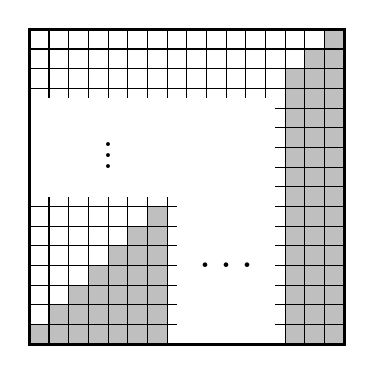
\begin{tikzpicture}[scale=0.5, x=0.5cm, y=0.5cm, font=\LARGE]
        \foreach \x in {0,...,15} 
            \foreach \y in {0,...,15}
                {
                    \pgfmathparse{(\x >= \y && (\x<7 || \x>12)) ? "lightgray" : "white"}
                    \edef\colour{\pgfmathresult}
                    \path[fill=\colour] (\x,\y) rectangle ++ (1,1);
                    \draw[black] (\x,\y) rectangle ++ (1,1);
                }
        \fill[white] (0, 7.5) rectangle ++ (8,5) node[color=black, pos=.5, align=center]{$\vdots$};
        \fill[white] (7.5, 0) rectangle ++ (5,8) node[color=black, pos=.5, align=center]{$\dots$};
        \fill[white] (7.5, 7.5) rectangle ++ (5,5) node[color=black, pos=.5, align=center]{$\iddots$};
        \draw[very thick, black] (0, 0) rectangle ++ (16,16);
    \end{tikzpicture}
\end{center}

现在,要求 $S(n)$ 的公式相当于求正方形内绘制的所有矩形覆盖区域的\emph{面积}。尝试将各个面积相加只是重述了这个问题,因此我们需要想办法将该面积与正方形的总面积联系起来。为此,我们要考虑剩下的是什么;也就是说,我们如何描述未被矩形覆盖的正方形的面积?看一下第一个 $1 \times 1$ 矩形正上方的区域:它也是一个矩形,尺寸为 $(n - 1) \times 1$。

看一下 $2 \times 1$ 矩形上方的区域:它是一个 $(n-2) \times 1$ 矩形。这种模式一直持续!最终,我们在 $(n - 1) \times 1$ 矩形上方有一个 $1 \times 1$ 矩形,并且最后一个 $n \times 1$ 矩形上方没有面积。所有这些矩形的总面积是多少?它看起来很像我们要求的 $S(n)$, 但它只是缺少最后一项 $n$。现在,我们可以将所有矩形的面积与 $S(n)$ 相关联,然后再与正方形面积相关联:
\[n^2 = S(n) + (S(n) - n) = 2S(n) - n\]
因此
\[S(n) = \frac{n^2+n}{2}\]
与我们之前得到的公式相同!

\subsubsection*{解题心得}

有时,有多种方法可以解决问题并得到最终解。有些可能很容易想到,但解起来很麻烦;有些可能很难想到,但解起来很容易;还些可能根本无济于事!通常很难事先判断任何特定方法会发生什么,所以只需动手尝试解题,看看会发生什么就可以了,跟踪你已经尝试过的内容和发生的情况,以便后面可以重新评估该方法。这是我们在数学生涯中需要牢记的一个事实。我们并不总能立即准确地知道该做什么。有时我们难免会陷入困境,或者最终走入死胡同。这不应该令人沮丧;事情就是这样!

作为一个子题,尝试为奇数 $n$ 的情况重做``配对'',但不要忽略求和的最后一项,而是尝试分离中间项并将数字从外到内配对。这是否会得出相同的结果?它看起来比我们使用的方法更容易/更快速/不同吗?或者,如果我们对于某个数字 $k$ 令 $n=2k$ 来处理偶数 $n$ 的情况会怎么样?对于奇数 $n$ 我们又该怎么办?这个符号会改变处理过程吗?会使它变得更容易处理吗? 现在,你能想出任何完全不同的方法来解决这个问题吗? 

\subsection{求和杂谈}\label{sec:section1.4.3}

\subsubsection*{奇数求和:观察模式}

既然谈到了整数求和,那就让我们来看一些相关的问题。首先,我们将介绍一种解释奇数之和的有趣得几何方法:让我们将 $1$ 表示为 $1 \times 1$ 块,然后将每个连续增大的奇数表示为角为 $1 \times 1$ 块的直角,完美贴合前一个这样的图。我们为什么要这样做?因为都是奇数,连续项的大小相差为 $2$,每次将角块的边延长 $1$,可以让直角与原图形紧密地相互贴合并逐渐构建起更大的正方形!

\begin{center}
    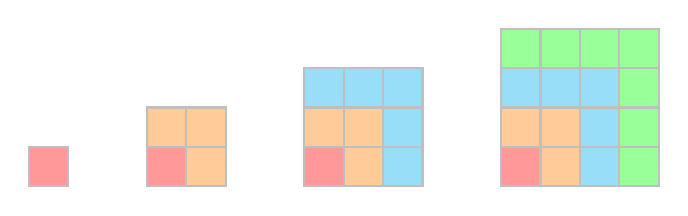
\begin{tikzpicture}[thick,scale=0.5, x=1cm, y=1cm]
        \foreach \x in {0,3,7,12}
        {
            \fill[red!40!white] (\x, 0) rectangle ++ (1,1);
            \draw[lightgray] (\x, 0) rectangle ++ (1,1);
        }

        \foreach \x in {3,7,12}
        {
            \foreach \i in {0,1}
            {
                \fill[orange!40!white] (\x+\i, 1) rectangle ++ (1,1);
                \draw[lightgray] (\x+\i, 1) rectangle ++ (1,1);
                \fill[orange!40!white] (\x+1, \i) rectangle ++ (1,1);
                \draw[lightgray] (\x+1, \i) rectangle ++ (1,1);
            }
        }

        \foreach \x in {7,12}
        {
            \foreach \i in {0,...,2}
            {
                \fill[cyan!40!white] (\x+\i, 2) rectangle ++ (1,1);
                \draw[lightgray] (\x+\i, 2) rectangle ++ (1,1);
                \fill[cyan!40!white] (\x+2, \i) rectangle ++ (1,1);
                \draw[lightgray] (\x+2, \i) rectangle ++ (1,1);
            }
        }

        \foreach \i in {0,...,3}
        {
            \fill[green!40!white] (12+\i, 3) rectangle ++ (1,1);
            \draw[lightgray] (12+\i, 3) rectangle ++ (1,1);
            \fill[green!40!white] (12+3, \i) rectangle ++ (1,1);
            \draw[lightgray] (12+3, \i) rectangle ++ (1,1);
        }
    \end{tikzpicture}
\end{center}

这种模式会持续下去吗?如果我们相信确实如此,我们如何证明这一点呢?这种几何图案的数值之和意味着什么?这是一个首先要回答的好问题,因为尽管几何图案很漂亮,但却很难使用和操作,最终也难以给出明确地\emph{证明}。本质上,对着模式的前几项说:``看,它有效!'' 并不构成官方的数学证明,因此我们必须找到更好的方法来表述这个问题。这并不是要淡化我们注意到的图案的意义和美丽;有趣的是,它的工作方式确实为我们提供了一些有价值的见解,让我们从数学上了解可能发生的事情,但归根结底,这就是它能为我们做的一切。

\subsubsection*{奇数求和:证明我们的发现}

让我们尝试用数字形式写出上图所表示的求和。 角块由 $1 \times 1$ 块组成,每个角比前一个多两块,因此我们看到的每个正方形都可以由一个和表示,例如
\[1 \:\text{ 或 }\: 1+3 \:\text{ 或 }\: 1+3+5 \:\text{ 或 }\: 1+3+5+7 \]
以此类推。我们从这些项中注意到,它们其实是平方数
\[1=1^2 \quad 1+3=4=2^2 \quad 1+3+5=9=3^2 \quad 1+3+5+7=16=4^2 \]
\emph{这}才是我们想要证明的模式;它相当于我们之前注意到的几何图案,但现在它是用我们可以操作的术语编写的。现在让我们思考一下如何才能做到这一点。这种模式与我们之前见过的模式相似吗?我们已经证明了关于整数和的结果了吗?当然!回顾之前的题目;(事实上,在某些方面)我们证明了
\[1 + 2 + 3 + \dots + (n_1) + n =\frac{n^2 + n}{2}\]
这对于该题有何用处?我们证明的求和公式涉及从 $1$ 到 $n$ 的\emph{所有}连续整数,但对于当前要求的公式,我们只想考虑连续\emph{奇数}。

之前我们用函数 $S(n)$ 表示前 $n$ 个自然数之和,所以我们定义函数 $T(n)$ 表示前 $n$ 个奇数之和。现在,我们首先需要确定该和的项,然后以某种方式将它们与 $S(n)$ 联系起来。下面,我们写出了 $n = 1,2,3 ,4$ 时的和。你能找到一种方法来识别求和中的最大项并用 $n$ 表示它吗?
\begin{align*}
    n=1: &\quad 1\\
    n=2: &\quad 1+3\\
    n=3: &\quad 1+3+5\\
    n=4: &\quad 1+3+5+7\\
\end{align*}
请注意,求和项的最后一项始终为 $2n-1$。这与一个普遍事实有关,即对于某个特定整数 $k$,任何偶数整数都可以表示为 $2k$,对于某个特定整数 $n$,任何奇数整数都可以表示为 $2n - 1$。(对于某个整数,我们也可以将奇数表示为 $2n + 1$,不过,这里使用 $2n - 1$ 更方便。)因此,我们要求的前 $n$ 个奇数之和的公式为
\[T(n) = 1 + 3 + 5 + 7 + \dots + (2n - 3) + (2n - 1)\]
我们可以将这个求和公式与 $S(n)$ 或类似的公式联系起来吗?请注意求和公式
\[S(2n) = 1 + 2 + 3 + \dots + (2n - 3) + (2n - 2) + (2n - 1) + 2n\]
包含从 $1$ 到 $2n$ 的\emph{所有}自然数,而 $T(n)$ 仅包含该范围内的奇数。也许两个和相减并尝试找到剩余项之和的表达式是有意义的:
\begin{align*}
    S(2n) - T(n) &= 1 + 2 + 3 + \dots + (2n - 1) + 2n \\
    &\quad -\big(1 + 3 + 5 + \dots + (2n - 3) + (2n - 1)\big) \\
    & =  2 + 4 + 6 + \dots + (2n - 2) + 2n
\end{align*}
这些项都是从 $2$ 到 $2n$ 的\emph{偶数}。我们怎样才能得到这个求和公式呢?我们是否需要做额外的工作,还是可以应用之前的证明结果?由于所有项都是\emph{偶数},我们可以将所有项除以 $2$ 并写成
\begin{align*}
    \frac{1}{2}\big(S(2n) - T(n)\big) &= \frac{1}{2}\big(2 + 4 + 6 + \dots + (2n - 2) + 2n\big)\\
    &= 1 + 2 + 3 + \dots + (n - 1) + n = S(n)
\end{align*}
我们可以保证,最右边的求和公式中的所有项都是整数。不仅如此,它们\emph{都是}从 $1$ 到 $n$ 的连续整数,并且我们知道它们的求和公式!现在,\text{一切都是用我们已知的公式}(即 $S(n)$ 和 $S(2n)$)以及我们要求的公式(即 $T(n)$)书写的。最后一步要做的是整理方程,分离 $T(n)$,然后代入我们已知的 $S$ 的公式:
\begin{align*}
    \frac{1}{2}\big(S(2n) - T(n)\big) &= S(n) \\
    S(2n) - T(n) &= 2S(n) \\
    T(n) &= S(2n) - 2S(n) \\
    T(n) &= \frac{(2n)^2 + 2n}{2} - \frac{2 \cdot (n^2 + n)}{2} \\
    T(n) &= \frac{4n^2 + 2n - 2n^2 - 2n}{2} \\
    T(n) &= \frac{2n^2}{2} \\ 
    T(n) &= n^2
\end{align*}
这看起来相当不错,不是吗?尽管必须完成一些代数步骤,我们还是得出了我们希望证明的结论:连续奇数的和是完全平方数。不仅如此,我们还成功地精确证明了该平方数与求和项数之间的关系。 具体来说,我们刚刚证明的结论的一种简洁概括描述是``前 $n$ 个奇数之和等于 $n^2$''。

\subsubsection*{另一种解法:归纳证明}

我们可以用不同的方式证明这一点吗?如果我们还没有证明上一节的结论,或者我们没有想到以这种方式证明它怎么办?我们能否以某种方式利用我们最初注意到的和的几何结构?

让我们回过头来用稍微不同的方式思考这个问题。具体来说,让我们看看为什么在求和中再添加一项会产生另一个平方数。假设我们已知其中一个求和产生一个平方数;我们知道这对于第一个求和 ($1 = 1^2$) 是正确的,但我们假设对于任意数量的项 $n$ 都会发生这种情况。也就是说,对于某个值 $n$, 我们\emph{假设}
\[1 + 3 + 5 + \dots + (2n - 3) + (2n - 1) = n^2\]
基于这一事实,我们接下来可以推断出下一个和是什么吗?当我们向求和中再添加一项时,我们会加上下一个奇数 $2n + 1$,所以让我们看看这会如何影响求和结果:
\[1 + 3 + 5 + \dots + (2n - 3) + (2n - 1) + (2n + 1) = n^2 + 2n + 1 = (n + 1)^2\]
这似乎证实了我们的想法,不是吗?知道求和的表现方式与我们预期的一致(``如果前 $n$ 个奇数整数之和为 $n^2$……'')我们就可以推断下一个和也必须以相同的方式表出现(……那么前 $n+1$ 个奇数整数的和是 $(n+1)^2$'')。这也证明了结论吗?你觉得怎么样?本质上假设我们的结论成立来进一步证明它,这感觉很奇怪吗?我们真的是这么做的吗?

这种证明策略 --- 使用结果的一种形式来证明结果的``后续''形式 --- 称为\textbf{数学归纳法}。(一般来说,``后续''一词的含义取决于上下文;在这里,它的意思是再加上一项后和。)我们将在下一章更详细地研究这一策略。目前,我们先指出这是一个完美的策略,但它高度依赖于第一个求和的正确表示:$1 = 1^2$。这样,我们所做的工作使我们能够推断出第二个求和是 $(1+3=2^2)$,接着就可以推断出第三个求和是 $(1+3+5=3^2)$,以此类推……如果我们只能证明第二部分,但第一部分的结果没有按照我们想要的方式计算怎么办?我们还能证明结论吗?一般来说,这对归纳策略有何启示?稍后我们将更普遍地解决其中一些问题。

\subsubsection*{泛化:算术级数}

我们要谈的最终求和问题与我们迄今为止看到的两个问题密切相关,事实上,如果我们能证明下一个结论,就不必证明前两个结论了!从这个意义上说,下一个结论比前两个结论更强:这个结论的真实性意味着前两个结论的真实性。(这是数学术语中的常见概念,将结论标记为比其他结论更强或更弱。)

对于这个结论,我们想要发展一个通用\textbf{算术级数}。这句话的意思是我们要添加一个算术级数,其中连续项之间的差是一个固定值。另一种思考方式是,每一项都是通过前一项加上一个固定常数而来。请注意,我们在后两个题目中求和的就是算术级数:第一个求和中,每项相差 $1$(或者,每项上加 $1$ 得到下一项),第二个求和中每个项相差 $2$(或者,每项上加 $2$ 得到下一项)。

我们如何表示一个通用的算术级数?因为连续项必须相差一个固定常数,让我们为该值分配一个变量,例如 $c$,作为常数。求和中也必须有第一项,所以让我们将该值分配给一个变量,例如 $a$,因为它是第一个字母。我们还需另一个变量来告诉我们求和中有多少项,因此我们将使用 $k$ 表示项数,因为我们之前已经使用过该变量表示相同的含义。现在,我们可以用这三个变量来表示整个求和:
\[A(a, c, k) = a + (a + c) + (a + 2c) + (a + 3c) + \dots + (a + (k - 2)c) + (a + (k - 1)c)\]
我们可以利用每对连续项相差 $c$ 这一事实,使用第一项 $a$ 来表示第二项,并且我们可以通过不断增加 $c$ 来表示第三项,依此类推。我们总共需要 $k$ 项,因此,将第一项视为 $a+ 0 \cdot k$,最后一项是我们将 $c$ 添加到第一项 $k - 1$ 次后得到的结果(从 $0$ 到 $k - 1$(含) 有 $k$ 个数字)。另请注意,我们引入了符号 $A(a, c, k)$ 来表示``第一项 $a$、常数差 $c$ 和 $k$ 项的算术级数之和''。现在,我们怎样才能算出这个和呢?

让我们采用以前有效的策略:在第一个求和题目中,我们正序和倒序写下求和项并将它们加在一起。这会创建许多具有相同求和结果的项对,从而将求和简化为乘法。如果我们在这里这样做时会发生什么?我们看到

\begin{center}
    \begin{tabular}{ccccccccc}
                 a & + &      (a+c) & + & \dots & + & (a+(k-1)c) & = & A(a,c,k)\\\noalign{\smallskip\smallskip}
        (a+(k-1)c) & + & (a+(k-2)c) & + & \dots & + &          a & = & A(a,c,k)\\\noalign{\smallskip\smallskip}
        \hline
        (2a+(k-1)c)& + & (2a+(k-1)c)& + & \dots & + &(2a+(k-1)c) & = &2A(a,c,k)\\\noalign{\smallskip\smallskip}
    \end{tabular}
\end{center}
我们再次发现配对项都有相同的和,在这种情况下,和是 $2a+ (k-1)c$。这样的配对项有多少对?正好是 $k$ 个项!(这就是我们选择使用该变量的原因。)将求和表示为乘法,我们现在可以推出
\[2A(a, c, k) = k \cdot (2a + (k - 1)c)\]
因此
\[A(a, c, k) = \frac{k}{2} \cdot k \cdot (2a + (k - 1)c)\]
这看起来符合你的期望结果吗?你的预期是什么?有时,尝试``猜测''可能会发生什么,然后看看结果是否与你的直觉相符,以及如何相符,会有所帮助。

\subsubsection*{具体应用}

上面提到过,我们之前题目中的求和都是算术级数,那么这个公式是否可以得出这些求和的正确结果呢?在第一题中,变量值为 $a = 1,c = 1, k = n$;代入这些值会得到
\[A(1, 1, n) = \frac{1}{2} \cdot k \cdot (2 + (n - 1)) = \frac{n}{2} \cdot(n+1) = \frac{n^2+n}{2}\]
这确实是我们之前得到的结论。那第二题呢?变量的值是多少?公式正确吗?这些问题请你来验证结果。

\subsubsection*{另一种表示}

这个问题的最后,我们想讨论另一种表示刚刚推导出的公式的方法。查看括号中的项,并以稍微不同的方式书写:$a+ (a+ (k-1)c)$。这些项看起来特别有趣吗?是的,它们分别是求和的第一项和最后一项。这为我们提供了一种不同的方式来表达我们推导出的求和公式:$A(a, c, k) = \frac{k}{2}(a + b)$,其中 $a$ 是求和的第一项,$b$ 是最后一项。这个版本的公式可以更方便,更快捷地进行一些求和。

例如,假如我们让你求一个算术级数之和,其中第一项为 $12$,最后一项为 $110$,总共有 $14$ 项,你就不必费心费力去计算常数差 $c$;相反,你可以简单地完成求和:$\frac{14}{2} \cdot (12 + 110) = 854$。是不是快得多?该算术级数的 $c$ 值是多少?给定 $a,b,k$,有没有一种简单的方法可以快速求出 $c$?

\subsubsection*{解题心得}

了解以前的结论会很有帮助,因为它们可以使证明更简短、更容易。有时,很难知道某个特定结果何时有用,或者即使意识到它的用途,也可能很难弄清楚如何应用它。在这种情况下,我们意识到到我们之前已经证明了一个求和公式,因此至少尝试弄清楚它在证明不同的求和公式时如何发挥作用是有意义的。然而,有一种完全不同的方法可以证明奇数之和的公式,不依赖于我们之前的结论。这暗示了一个更通用的结论,好奇的数学家会尝试更通用地探索这个问题,我们通过研究任意算术级数做到了这一点。但最终,我们对前两个求和公式使用了多种策略,并且仅将其中一种策略应用于一般级数问题。我们可以在其他设定下使用这些策略吗?我们是否也可以通过归纳法来证明第一个求和公式?我们可以使用正序/逆序技术来证明第二个求和公式吗?尝试使用这些策略,看看会发生什么。这对你来说可能会很奇怪或没有必要,因为我们已经有了结论,但是了解不同技术在不同环境中如何发挥作用是一个宝贵的经验。在数学中,弄清楚在证明中使用哪种策略通常与找出证明结果一样困难(甚至更难)。考虑到这一点,练习特定的策略来培养一种直觉,知道它们何时有效以及何时需要尝试其他方法,是很有帮助的。

\subsection{好友倾向}

\subsubsection*{问题描述}

这个问题基于以下一则关于匈牙利社会学家的轶事以及他对儿童朋友圈的观察。

\begin{quote}
    ``20 世纪 50 年代,匈牙利社会学家 S. Szalai 研究了儿童之间的友谊关系。他观察到,在任何大约 $20$ 个孩子的群体中,都能找到四个孩子是共同的朋友,或者四个孩子中没有两个孩子是朋友。在得出社会学结论之前, S. Szalai 咨询了当时三位著名的匈牙利数学家: Erdos, Turan 和 Sos 。简短的讨论后表明,这其实是一种数学现象,而非社会学现象。对于至少 $18$ 个元素上的任意对称关系 $R$,存在 $4$ 个元素的子集 $S$,使得 $R$ 包含 $S$ 中的所有对或不包含其中任何对。这一事实是 1930 年证明的拉姆齐定理(Ramsey's theorem)的一个特例,拉姆齐理论的基础,后来发展成为组合数学的一个丰富领域。 --- (引自麻省理工学院 Jacob Fox 教授的\href{https://www.a.com}{讲义}。)''
\end{quote}

现在我们遵循相同的思路提出类似的问题,但数字较小。具体来说,我们想要找出\emph{满足}其中三人相互都是朋友或敌人的最小群体规模。

\begin{quote}
    假设在一群人中,其中任意两人要么是朋友,要么是敌人,并且这是唯一可能的关系(即没有熟人或亦敌亦友或类似的关系)。以四人为一组,试着为每对指定朋友/敌人关系,使得不会有三人一组都是朋友或敌人。五个人可以实现吗?六个呢?七个?十个?二十个呢?尝试确定最小群体规模,使得你就可以\emph{保证}找到一个由三个人组成的小组,他们要么都是朋友,要么都是敌人。
\end{quote} 

请仔细思考一下,然后再翻页阅读解答。

\clearpage

\subsubsection*{有效地表述问题}

你做出来了吗?这是一个非常棘手的问题,所以如果你没有解出来,请不要感到难过。事实上,我们认为调查这个问题与实际找到答案一样重要,因为有多种方法可以解决这个问题,而且看不同的人如何解释这个问题总是很有趣。

首先,让我们讨论一下如何写下/画出/谈论这种情况。对于该题提出的任何问题,我们都应该考虑一组具有一定规模的人,并思考这群人中任意两人之间的关系。为了解决这个问题,我们需要一种高效且易于解释的方法表示所有这些关系,以便我们可以验证大小为 $3$ 的子群所需的属性。具体来说,我们想要轻松识别是否存在大小为 $3$ 的\emph{同质}子群,即三个人\emph{互为}朋友或\emph{互为}敌人。从现在起,我们将其称为``\textbf{同质性}''。

我们怎么才能做到这一点呢?我们如何才能表示人及其关系呢?我们可以对小组中的人员进行编号,然后写出所有数字对的列表,并用 $F$(朋友)或 $E$(敌人)标记每对数字的关系。让我们尝试为四人小组执行此操作:

\[12F \quad 13E \quad 14F \quad 23F \quad 24E \quad 34F\]

这群朋友/敌人满足同质性吗?验证起来并不那么容易,不是吗?首先,编号使得很难找到大小为 $3$ 的子群,为了验证属性,我们需要检查所有此类子群以确保它们不是 $E E E$ 或 $F F F$。也许在尝试解决问题之前,我们应该找到一种更好的方式来表示信息。对于群体中的所有可能配对,你能想出一种视觉上令人更加愉悦的方式来表示两个人是朋友还是敌人吗?具体来说,我们希望得到一种相对有效的方法来寻找大小为 $3$ 的子群并识别它们是否全是朋友还是全是敌人。

让我们尝试将组中的每个人表示为一个点,并根据这两个人是朋友还是敌人用一种线连接两个人。例如,我们用蓝线表示朋友,用红线表示敌人(记住,任何两个人要么是朋友,要么是敌人,没有别的可能,所以每对点必然有彩色线连接它们)。例如,下图描述了我们在上面分配的关系和符号:

\begin{center}
    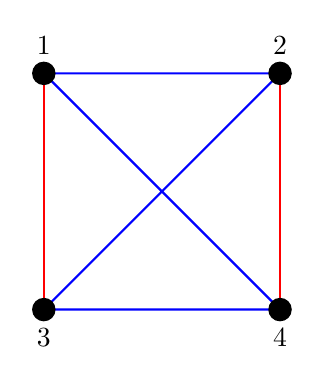
\begin{tikzpicture}[thick,scale=0.5]
        \coordinate (A) at (0,6);
        \coordinate (B) at (6,6);
        \coordinate (C) at (0,0);
        \coordinate (D) at (6,0);
        \draw[blue] (A) node[black, above, yshift=3pt]{$1$}
        -- (B) node[black, above, yshift=3pt]{$2$}
        -- (C) node[black, below, yshift=-3pt]{$3$}
        -- (D) node[black, below, yshift=-3pt]{$4$}
        -- (A);
        \draw[red] (A)--(C);
        \draw[red] (B)--(D);
        \foreach \n in {A,B,C,D}
            \node at (\n)[circle,fill,inner sep=3pt]{};
    \end{tikzpicture}
\end{center}

现在,我们要用什么方法来验证同质性?我们需要三个点(三个人),使得它们之间的所有线都是蓝色(都是朋友)或红色(都是敌人)。没错 --- 我们寻找的正是\textbf{单色三角形}!(注意:我们希望三角形的顶点是我们绘制的原始点;也就是说,我们不希望顶点是两条线的交点。此外,\emph{单色}来自希腊语 \emph{monos} 和 \emph{khroma},分别表示``一个''和``颜色''。)这种表示方式更容易直观地解释,并且可以更快地检验。

根据上图,我们解决了四人组问题:我们找到了朋友和敌人的特定排列,因此不存在全为朋友或全为敌人的三人组。也就是说,不存在具有同质性的大小为 $3$ 的子组。这表明这样的情况可以用四个人来实现,因此我们不能\emph{保证}四个人之间一定存在具有同质性的组。

你还能找到另一个这样的排列吗?你如何确定这与我们已经看到的排列\emph{不同}?有多少种不同的排列满足同质性?现在,尝试绘制一个排列,该排列\emph{一定}具有大小为 $3$ 且具有同质性的子组。那看起来会是什么样?这样的排列有多少种?

\subsubsection*{重述 $n = 5$ 的问题}

让我们继续思考由五个人组成的小组。我们的图需要发生改变,因为我们现在有五个点,这意味着需要绘制更多的线。尽管如此,我们还是会用蓝色或红色线填充所有连接,并确保没有单色三角形。这可能吗?(提示:尝试将点排列成规则的五边形形状,然后填充线。)尝试画几次,看看你的排列是否有效。随机画几条线,然后通过确保添加的新线不会创建单色三角形来指导你的选择,这也可能有帮助。

你做出来了吗?翻页看看我们是如何做的...

\clearpage

\subsubsection*{解答:$n=5$}

这是我们在五个点之间排列的红/蓝线,完全避免了同质性:

\begin{center}
    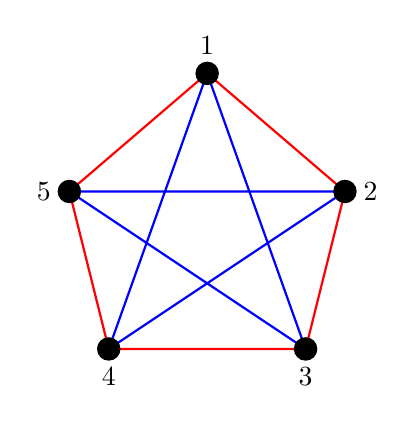
\begin{tikzpicture}[thick,scale=0.5]
        \coordinate (A) at (0,0);
        \coordinate (B) at (5,0);
        \coordinate (C) at (6,4);
        \coordinate (D) at (2.5,7);
        \coordinate (E) at (-1,4);
        \draw[red] (A) node[black, below, yshift=-3pt]{$4$}
        -- (B) node[black, below, yshift=-3pt]{$3$}
        -- (C) node[black, right, xshift=3pt]{$2$}
        -- (D) node[black, above, yshift=3pt]{$1$}
        -- (E) node[black, left, xshift=-3pt]{$5$}
        -- (A);
        \draw[blue] (A)--(D)--(B)--(E)--(C)--(A);
        \foreach \n in {A,B,C,D,E}
            \node at (\n)[circle,fill,inner sep=3pt]{};
    \end{tikzpicture}
\end{center}

请注意该图形优雅的对称性:所有红线均位于五边形的外侧,所有蓝线均位于该形状的内部。这样做的原因是,任意三个相邻点作为顶点的三角形必须使用两条外线和一条内线,任意三个不相邻点作为顶点的三角形必须使用两条内线和一条外线。(想一想:为什么我们不能用三条内线或三条外线来组成一个三角形?)这\emph{保证}了我们绘制的任何三角形都会使用两条不同颜色的线,所以这个图形不具有同质性!当然,我们可以查看图中所有可能的三角形,并确保它们都不使用一种颜色。这样的三角形有多少个?你能多快手工找到所有这些三角形?这样做是否更容易,或者注意我们上面提到的内部/外部属性?

也许你找到的解决方案与我们的图不同。你怎么知道它实际上是否是不同的图形?你的图中有多少条蓝线、多少条红线?我们的图呢?尝试通过移动点来重新绘制图形,但保持点之间的关系(即任意两个点之间绘制的线条的颜色)。你能把你的图形弄得跟我们的一样吗?你认为这对本题解的数量意味着什么?

\subsubsection*{$n=6$ 的情况}

好的,现在我们可以思考六个人的情况了。就点和线而言,我们希望用蓝色或红色线绘制六个点之间所有可能的连接,并确保不存在边都为相同颜色的三角形。在绘制前,请思考四个点和五个点时我们的解决方案。这些解是什么样的?这次我们要画多少线?我们可以试着让这个数字看起来像五个点的解决方案吗?有时,思考当前问题的解决方案与以前工作有何相似之处会大有帮助。现在,尝试画出这个图形,看看会发生什么。

有效吗?为什么无效?你在哪里遇到了麻烦?在不得不绘制单色三角形之前,你可以画多少条线?也就是说,在你绘制下一条线形成单色三角形之前,无论它是蓝色还是红色,你可以向图形中插入多少条线?某种程度上,这些问题对于解决这个特定难题来说是无关紧要的问题,但它们值得思考,因为它们本身很有趣,并且它们可能会引导我们找到这个难题的解决方案或其概括。为了便于说明,这是我们在图形中分配红线和蓝线的一种方案。我们为什么停在这里?还需要添加多少条线?我们能加进去吗?

\begin{center}
    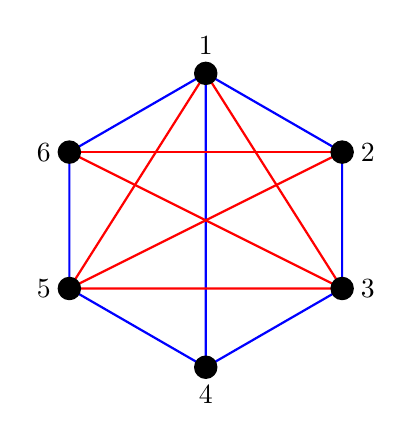
\begin{tikzpicture}[thick,scale=0.5]
        \coordinate (A) at (0,0);
        \coordinate (B) at (-3.4642,2);
        \coordinate (C) at (-3.4642,5.4642);
        \coordinate (D) at (0,7.4642);
        \coordinate (E) at (3.4642,5.4642);
        \coordinate (F) at (3.4642,2);
        \draw[blue] (A) node[black, below, yshift=-3pt]{$4$}
        -- (B) node[black, left, xshift=-3pt]{$5$}
        -- (C) node[black, left, xshift=-3pt]{$6$}
        -- (D) node[black, above, yshift=3pt]{$1$}
        -- (E) node[black, right, xshift=3pt]{$2$}
        -- (F) node[black, right, xshift=3pt]{$3$}
        -- (A)
        -- (D);
        \draw[red] (B)--(E);
        \draw[red] (C)--(F);
        \draw[red] (B)--(D)--(F)--(B);
        \draw[red] (C)--(E);
        \foreach \n in {A,B,C,D,E,F}
            \node at (\n)[circle,fill,inner sep=3pt]{};
    \end{tikzpicture}
\end{center}

我们现在面临的情况很有趣,因为它与我们之前面临的情况性质相反。在四个点和五个点的情况中,我们想表明\emph{可以}通过排列所有线来消除单色三角形。为了证明这一点,只需画出来就好!画出具有所需属性的\emph{特定}图形就足以证明可以实现我们想要的属性。然而,对于六个点,似乎不可能将线条排列得不存在单色三角形。我们怎样才能证明这是事实呢?我们很容易想到,只需考虑线条的所有可能排列,并论证每一中排列中至少有一个单色三角形。这可行吗?线条有多少种排列方式?我们如何在任意给定图形中轻松找到单色三角形?还记得我们对五个点的图形进行此操作吗?我们注意到,任何三角形都必须使用\emph{至少}一条来自外部的线和\emph{至少}一条来自内部的线,这保证了任何三角形都有两种类型的线。我们可以在这里做同样的事情,并明确一些\emph{保证}存在非单色三角形的性质吗?

问题是,图中六点之间线的可能排列方式太多了,我们无法手动完成所有检查!这里有 $15$ 条线需要绘制,每条线都可以是蓝色或红色,因此共有 $2^{15}$ 种可能的排列。这是一个很大的数字!(实际上,排列可能性会稍微少一些,因为其中一些排列在某种意义上是等价的;更专业地说,它们是``\emph{同构的}''。)

\subsubsection*{解答:处理\emph{任意}图形}

我们需要更巧妙地进行论证,这样我们就可以在不绘制特定图形的情况下证明\emph{任意}图形的性质。也就是说,我们需要找到一些事实,一些对所有可能的六点图都成立的性质,但我们仍然能够推断出一定存在三角形。解决这个问题的一种方法是考虑在图形的一小部分中绘制线条。具体来说,让我们取六个点中的任意一个,并考虑从该点引出的五条线。例如,我们可能会得到下面的图形:

\begin{center}
    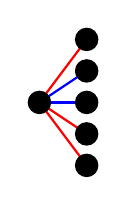
\begin{tikzpicture}[thick,scale=0.2]
        \coordinate (A) at (0,0);
        \coordinate (B) at (3,2);
        \coordinate (C) at (3,0);
        \coordinate (D) at (3,4);
        \coordinate (E) at (3,-2);
        \coordinate (F) at (3,-4);
        \draw[blue] (A)--(C);
        \draw[blue] (A)--(B);
        \draw[red] (A)--(D);
        \draw[red] (A)--(E);
        \draw[red] (A)--(F);
        \foreach \n in {A,B,C,D,E,F}
            \node at (\n)[circle,fill,inner sep=3pt]{};
    \end{tikzpicture}
\end{center}

有多少蓝线,多少红线?这在一定程度上是一个棘手的问题:我们并没有真正考虑任何\emph{特定}图形(如上面的图形),而是试图找到有关所有可能图形的事实。因此,我们不能太具体地回答这个问题。假设我们看到一个\textbf{任意}图形,我们必须提出一个无论该图形是什么都有效的论证。 

我们\emph{可以}这样说:必须至少有三条蓝线或三条红线。你明白为什么这是真的吗?使其不成立的唯一方法是从特定点出发,有两条(或更少)蓝线和两条(或更少)红线,共计四条(或更少)线。不过,我们必须画出所有可能的连接,因此应该有五条!(这个论证是``\emph{鸽笼原理}''的一个例子。这个原理说的是,我们无法将两种不同颜色的五个物体放入两个不同盒子中,而不将三个同种颜色的物体放入一个盒子。对这类问题来说,鸽笼原理是一个非常有用的策略,我们稍后将在 \ref{sec:section8.6} 节更详细地研究该原理。)

那么我们的立场是什么呢?我们从任意一个六个点、填满线的图形开始,到专注于一个特定的点;从这个点出来,一定有三条蓝线或三条红线。它可以是任意一种颜色,所以我们不能仅仅假设它是红色的并遵循这种假设进行论证;我们可以这样做,但之后必须回到这一点,看看如果这三条线是蓝色的,会发生什么变化。因此,让我们这样处理:让我们检查所有有三条红线从该特定点引出的图形。我们能得到什么?我们还没有对图中的其他线做出任何假设,所以让我们看看它们可能是什么。观察下图,看看到目前为止我们假设存在哪些线条颜色:

\begin{center}
    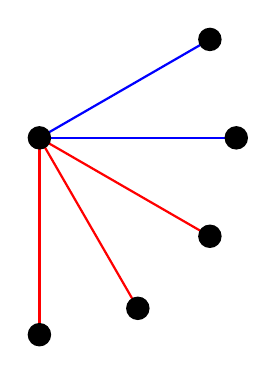
\begin{tikzpicture}[thick,scale=0.5]
        \coordinate (A) at (0,0);
        \coordinate (B) at (4.33,2.5);
        \coordinate (C) at (5,0);
        \coordinate (D) at (4.33,-2.5);
        \coordinate (E) at (2.5,-4.33);
        \coordinate (F) at (0,-5);
        \draw[blue] (A)--(C);
        \draw[blue] (A)--(B);
        \draw[red] (A)--(D);
        \draw[red] (A)--(E);
        \draw[red] (A)--(F);
        \foreach \n in {A,B,C,D,E,F}
            \node at (\n)[circle,fill,inner sep=3pt]{};
    \end{tikzpicture}
\end{center}

现在,可以在该图中添加哪些线而不会在三点之间形成同种颜色的三角形?我们不能对图中两个孤立点之间的线做任何假设,所以让我们关注底部的三个点。其中的线条可能是什么颜色?如果其中任何一条是红色的,那就会在该线的两个端点和我们关注的原始点之间形成一个单色三角形!这是有问题的。

\begin{center}
    \begin{tikzpicture}[thick,scale=0.5]
        \coordinate (A) at (0,0);
        \coordinate (B) at (4.33,2.5);
        \coordinate (C) at (5,0);
        \coordinate (D) at (4.33,-2.5);
        \coordinate (E) at (2.5,-4.33);
        \coordinate (F) at (0,-5);
        \draw[blue] (A)--(C);
        \draw[blue] (A)--(B);
        \draw[red] (A)--(D);
        \draw[red] (A)--(E);
        \draw[red] (A)--(F);
        \draw[red] (E)--(F);
        \draw [red,-stealth,very thick] (-2,-2.4) node[red, above]{$\text{红色三角形}$} -- (1,-3.5);
        \foreach \n in {A,B,C,D,E,F}
            \node at (\n)[circle,fill,inner sep=3pt]{};
    \end{tikzpicture}
\end{center}

避免这种情况的唯一方法是将所有这些线都变成蓝色。但这会在这三个点之间形成一个蓝色三角形!哇,看来无论我们做什么都无法避免生成单色三角形!

\begin{center}
    \begin{tikzpicture}[thick,scale=0.5]
        \coordinate (A) at (0,0);
        \coordinate (B) at (4.33,2.5);
        \coordinate (C) at (5,0);
        \coordinate (D) at (4.33,-2.5);
        \coordinate (E) at (2.5,-4.33);
        \coordinate (F) at (0,-5);
        \draw[blue] (A)--(C);
        \draw[blue] (A)--(B);
        \draw[red] (A)--(D);
        \draw[red] (A)--(E);
        \draw[red] (A)--(F);
        \draw[blue] (F)--(D)--(E)--(F);
        \draw [blue,-stealth,very thick] (5.5,-3.8) node[blue, right]{$\text{蓝色三角形}$} -- (2.5,-3.8);
        \foreach \n in {A,B,C,D,E,F}
            \node at (\n)[circle,fill,inner sep=3pt]{};
    \end{tikzpicture}
\end{center}

让我们回到鸽笼理论并重新评估情况。如果原理保证的相同类型的三条线是蓝色而不是红色会怎样?其实,不会有什么改变。向图形底部的三个点之间添加新线,我们仍然会陷入困境:

\begin{center}
    \begin{tikzpicture}[thick,scale=0.5]
        {
            \coordinate (A) at (0,0);
            \coordinate (B) at (4.33,2.5);
            \coordinate (C) at (5,0);
            \coordinate (D) at (4.33,-2.5);
            \coordinate (E) at (2.5,-4.33);
            \coordinate (F) at (0,-5);
            \draw[red] (A)--(C);
            \draw[red] (A)--(B);
            \draw[blue] (A)--(D);
            \draw[blue] (A)--(E);
            \draw[blue] (A)--(F);
            \draw[blue] (E)--(F);
            \draw [blue,-stealth,very thick] (-2,-2.4) node[blue, above]{$\text{蓝色三角形}$} -- (1,-3.5);
            \foreach \n in {A,B,C,D,E,F}
                \node at (\n)[circle,fill,inner sep=3pt]{};
        }
        {
            \coordinate (A1) at (8,0);
            \coordinate (B1) at (12.33,2.5);
            \coordinate (C1) at (13,0);
            \coordinate (D1) at (12.33,-2.5);
            \coordinate (E1) at (10.5,-4.33);
            \coordinate (F1) at (8,-5);
            \draw[red] (A1)--(C1);
            \draw[red] (A1)--(B1);
            \draw[blue] (A1)--(D1);
            \draw[blue] (A1)--(E1);
            \draw[blue] (A1)--(F1);
            \draw[red] (F1)--(D1)--(E1)--(F1);
            \draw [red,-stealth,very thick] (13.5,-3.8) node[red, right]{$\text{红色三角形}$} -- (10.5,-3.8);
            \foreach \n in {A1,B1,C1,D1,E1,F1}
                \node at (\n)[circle,fill,inner sep=3pt]{};
        }
    \end{tikzpicture}
\end{center}

如果我们加入任何蓝色线,它就会与原始点形成一个单色三角形,如果我们将它们全部变成红色,就会在那三个点间形成一个单色三角形!从这个意义上讲,我们在鸽笼理论之后遵循的两个论证是\emph{相同的}。如果我们用``红色''替换``蓝色''一词,反之亦然,我们会得到相同的论点。有时,数学家会利用这种情况来简化证明,只说``不失一般性,三条线是红色的''。这通常意味着,如果我们做出其他选择(即,如果线是蓝色的),那么进一步的论证在数学上将具有相同的结构,因此我们可以不重复书写相同的文字来节省时间和空间。事实上,这种情况非常常见,以至于有时你可能会看到``不失一般性''这个短语缩写为 \textbf{WOLOG} 或 \textbf{WLOG}。

\subsubsection*{解答:总结结果}

到目前为止我们取得了什么成果?我们绘制了\emph{特定}的图形,表明我们可以将线条排列在四个和五个点之间,而不出现单色三角形,并且我们认为\emph{任何}由六个点构成的图\emph{一定}具有单色三角形。就题目中朋友/敌人的表述而言,这意味着任何六人组必然存在一个三人组,其中的成员要么都是朋友要么都是敌人。

请注意,把这个问题改写成这个点/线的形式是多么有帮助;它让我们完全忘记了问题的社交背景(某种程度上,这可能会分散注意力),并简化了术语和符号(我们将成对的人标记为``朋友''或``敌人''变为简单地绘制两点之间一条线)。这是一个非常有用的策略:提取谜题的内在结构 --- 底层工作、元素之间的关系、它们如何相互作用等 --- 并根据这些部分重写所有内容。这可以使难题变得更容易理解和解决,并且可以指导我们设计更好的符号。如果我们继续用 $13F, 23E, \dots$ 这种符号来解决这个问题会怎样?也许最终能解决,但会困难得多!

这个题目最初的问题之一是确定一个下界,使得任何更大的人群都必然拥有该子群属性。你认为我们已经做到了吗?我们确定了一个下界了吗?六可能是这个数字吗?为什么是或为什么不是?在任意七人组中,都有一个较小的六人组,而我们上面的工作证明该小组中必然存在三个共同的朋友/敌人!当然,这适用于任何人数超过六人的群体,因此这一定是我们要寻找的精确下界。这与题目原始陈述中提到的结果类似,匈牙利社会学家在规模为四的子群中注意到了这种现象。这个问题解决起来要困难得多,所以我们这里解决了一个更小、更简单的案例。这两个结果都与称为\textbf{拉姆齐理论}的一大类问题有关。组合学和图论的这个分支致力于识别这些``下界'',随着某种结构(如一群人)的规模不断增长,最终会出现一个点,我们可以\emph{保证}找到一个具有某种属性的子群(三个共同的朋友/敌人)。起初被认为是一种社会学现象,后来被证明是严格的数学事实。牛不牛!

\subsubsection*{泛化:留给你的问题}

在继续之前,让我们提出一些有趣且相关的问题。如果我们要寻找不同规模的同质群(例如四个、五个或十二个)该怎么办?当然,总的来说,我们必须有更多的人才能保证找到这样的子群。我们可以一直这样做吗?也就是说,给定任何所需的子群大小,我们可以像上面那样确定一个下界吗?即使没有找到特定的数字,你能想出如何证明这样的下界一定存在吗?此外,如果我们允许第三种可能:朋友、敌人、陌生人,又会怎样呢?我们可以回答关于同质群的类似问题吗?这些都与拉姆齐理论相关,甚至其中一些问题相当难以回答,需要数学家多年努力才能解决。许多此类简单问题仍然是悬而未决的、未解难题!如果你在这些问题上没有任何进展,请不要灰心。我们相信,对这些问题的任何尝试和思考都是有意义且有益的。

\subsubsection*{解题心得}

这个问题带来了几个困难。首先,我们必须找到一种方法来以有意义的方式解释谜题,以便我们可以解决这个问题,这涉及到提出适当的符号来表示题目的元素。这是解决数学问题的重要组成部分,特别是这种不将符号和可视化作为问题陈述一部分的问题。

其次,为了确定 6 是群规模下界,我们必须以某种方式证明某些事情是\emph{不}可能的,但要检验的可能情况数量太大,无法单独检验每种情况。这种情况经常发生,特别是在与计算机科学和算法相关的问题中。为了解决这个问题,我们必须采用一种比大力出奇迹更巧妙的策略,而且并不总是清楚该采取什么策略。在这里,我们先是尝试填入线,就好像它会成功一样,然后意识到我们已经达到了一个无法添加的地步。证明某件事是可能的,相当于只是展示该现象的一个例子(我们对四人和五人组就是这么做的),但证明某件事是\emph{不可能}的可能要棘手得多,并且需要一些依赖上下文的独创性。

最后,我们发现,思考与当前问题密切相关的问题可能会很有趣,这些相关问题往往只需调整原问题的一个或多个条件。如果我们寻找更大的子群怎么办?如果我们允许更多类型的线怎么办?这将如何改变结果?通过改变这些条件来探索问题的边界可以带来新的数学发现和技术,并促使数学家积极探寻新的知识和分享知识的方法。

\clearpage

\subsection{三门问题}

\subsubsection*{问题描述}

这个问题只涉及基本的概率和算术,但多年不断有非常聪明的人在这道题上折戟沉沙。事实上,1990 年,玛丽莲·沃斯·萨万特 (Marilyn vos Savant) 在《Parade》杂志的专栏中发表了这个问题及其解法,引发了一场争论,许多人(包括数学家)写信表示赞同或反对她(应该说是正确的)答案。让我们看看你的想法!

\begin{quote}
    假设你正在参加一个游戏节目,有三扇门供你选择。其中一扇门后面是汽车;其余的后面是山羊。游戏前,汽车和山羊被随机放置在门后。游戏节目规则如下:选择一扇门后,该门暂时保持关闭状态。游戏节目主持人蒙蒂·霍尔(Monty Hall)知道门后有什么,他会打开剩下两扇门中的一扇,并且打开的门后面一定是山羊。如果剩下的两扇门后面都是山羊,他会随机打开一扇。蒙蒂·霍尔打开一扇有山羊的门后,他会问你是继续选择最初选择的门还是切换到剩下的另一扇门。想象一下,加入你选择了 1 号门,主持人打开了 3 号装有山羊的门。然后他问你``你想换到 2 号门吗?'' 改变你最初的选择对你有利吗?
\end{quote}

当然,我们假设你更愿意赢得一辆汽车而不是一只山羊,并且你希望最大化赢得那辆车的机会。 另外,值得一提的是,这个问题的名字来源于电视游戏节目《\emph{Let's Make a Deal}》的主持人蒙蒂·霍尔(Monty Hall)。

所以你怎么看?想象一下你站在电视观众面前的舞台上,当蒙蒂·霍尔问你:``你想换到另一扇门吗?'' 你会怎么选择?

请仔细思考一下,然后再翻页阅读解答。

\clearpage

\subsubsection*{解答:始终切换}

我们先直接给出答案,因为这可能会让你大吃一惊:你绝对应该改变最初的选择!推理并得到这个答案是棘手和令人困惑的部分,而建立正确的解释该题的方法是困扰求解者这么长时间的部分原因。

\subsubsection*{分析错误论证}

首先让我们向你演示一个错误的``解答'',该解答声称切不切换无关紧要。想象一下你和你的朋友听到了这个问题,他/她给了你这么一个解释。你会如何回应?你同意吗?为什么?如果不是,你会如何指出他们的错误?他们的解释有什么问题?

\begin{quote}
    当我选择了一扇门,蒙蒂·霍尔向我展示了另一扇后面有山羊的门,那么就只有两扇门没有打开。其中一扇是山羊,另一扇是汽车,所以汽车在我选择的门后面的可能性是 $50/50$,汽车在另一扇门后面的可能性也是 $50/50$。所以,换不换都无所谓,还不如坚持最初的选择。
\end{quote}

上面的解释说服你了吗?让我们试着找出这个论证的问题。为了解决这个难题,我们需要解决的主要问题是计算出两个数字:坚持我们最初的选择赢得汽车的概率,以及切换到另一扇门后赢得汽车的概率。我们需要识别这两个值并进行比较;只有这样我们才能明确地解决这个难题。

上面的论证似乎通过说这两个概率都是 $50\%$ 来解决这问题,但反对者如何解释这种情况存在问题。你认为坚持最初的选择赢得汽车的概率有多大?本质上讲,这相当于蒙蒂·霍尔没有向我们展示另一扇后面有山羊的门。如果我们坚持对门的最初选择,我们甚至可能不会看到另一扇后面有山羊的门,因为这不会影响我们最初选择的门后面的物体。让我们重申这个想法以强调其重要性:

\begin{quote}
    因为有三扇门,所以一开始选择正确的门的概率是 $\frac{1}{3}$,看到另一扇门后面有山羊\emph{并不能改变这一事实}。
\end{quote}
这就是上面论证的问题,事实上,这是``解答''这个问题时最常见的错误之一。

下一步是计算切换后赢得汽车的概率,并将其与 $\frac{1}{3}$ 进行比较。事实上,有多种方法可以实现这一目标。一种简洁的方法是,每当我们初次选择的门后碰巧是山羊时,切换就会成功(赢得汽车)。这种情况下,两扇未选择的门按某种顺序隐藏了山羊和汽车,游戏节目主持人被迫向我们展示山羊;因此,汽车隐藏在剩下的门后面,切换就会获胜。由于我们的初次选择在 $\frac{2}{3}$ 的情况下会选到有山羊的门,因此我们得出结论,$\frac{2}{3}$ 的情况下切换会赢得汽车。

\subsubsection*{枚举可能性}

上面的解释可能无法令你满意,所以让我们尝试实际枚举(明确计算)门后山羊和汽车的可能排列,并写下如果我们在每种情况下进行切换会发生什么。首先要注意的是,门的编号是无关紧要的,因为所有选择都是随机做出的;也就是说,无论汽车停在印有``1 号''的门后,还是``2 号''或``3 号'',结果都是一样的:我们仍然有 $\frac{1}{3}$ 的概率选到那扇有车的门。 因此,我们可以假设\textbf{WOLOG}(记住这个缩写的意思是``不失一般性'')汽车位于 1 号门后面,山羊站在 2 号门和 3 号门后面。当然,这是我们对问题的强加,我们不能说玩家知道这一点(否则他/她每次都会选择1 号门!)。按照这种安排,让我们检验一开始可以做出的所有 $3$ 个选择,看看在每种情况下切换或坚持会有什么效果:

\begin{center}
    \begin{tabular}{ c|c|c } 
     1 号门 & 2 号门  & 3 号门 \\ 
     \hline 
     汽车   & 山羊    & 山羊 \\
    \end{tabular}
\end{center}

\begin{center}
    \begin{tabular}{ c|c|c|c } 
     我们的选择 & 主持人展示 & 换门结果 & 不换门结果 \\ 
     \hline 
     1 号门    & 2 号门 \:或\: 3 号门  & 山羊 & 汽车 \\
     2 号门    & 3 号门            & 汽车 & 山羊 \\
     3 号门    & 2 号门            & 汽车 & 山羊 \\
    \end{tabular}
\end{center}

一个重要的观察是,当我们最初选中有汽车的门时,主持人可以选择剩余的门中的任意一个展示山羊,并且他会\emph{随机}做出选择。然而,无论选择展示哪扇门,我们都会因为切换而失败,因为坚持而获胜。尽管如此,这种情况只占 $\frac{1}{3}$,即我们最初选中了后面有汽车的门。由于上表中每一行的可能性相同,我们可以得出结论,$\frac{2}{3}$ 的情况下我们会因为切换而获胜,而 $\frac{1}{3}$ 的情况下我们会因为坚持而获胜。

现在这个问题是不是更合理了?尝试向你的朋友和家人提出这个问题,并测试他们的反应。有多少人给出了正确答案?有多少人能正确给出解释?有多少人错误地说``无所谓''?有多少人之前已经听说过这个问题?

\subsubsection*{泛化到许多门许多车}

让我们泛化一下这个游戏节目的情况,并尝试证明切换是否仍是一个好主意。具体来说,假设总共有 $n$ 扇门和 $m$ 辆汽车,因此有 $n - m$ 只山羊。为了分析这一点,我们需要指定 $m \le n - 2$。思考为什么这是必要的:

\begin{itemize}
    \item 如果 $m = n$,那么无论是否切换,我们总是会赢。因此,这种情况没有什么可以证明的。
    \item 如果 $m = n-1$,那么如果我们一开始碰巧选中后面有山羊的门,主持人就\emph{无法}向我们展示另一扇有山羊的门。因此,游戏规则遭到破坏,切换不切换也就毫无意义。
\end{itemize}

现在,有了这些变量,游戏的新规则如下:我们选择 $n$ 扇门中的一扇。主持人从所有\emph{其他}门中找出藏有山羊的门,并随机打开其中一扇门。然后,我们可以选择坚持原来的选择或切换到\emph{任意}其他门。现在的策略是什么?我们应该切换吗?我们应该坚持吗?答案完全取决于 $m$ 和 $n$ 吗?为什么?

我们将用与原题中第一种方法大致相同的方式来处理这个修改后的问题。我们不可能枚举这个版本中的所有情况,因为 $m$ 和 $n$ 是未知变量。相反,我们需要应用逻辑推理来推断坚持和切换的获胜概率。第一个关键观察与我们之前所做的完全相同:\emph{坚持}获胜的概率正是首次选中藏有汽车的门的概率。当我们首次选中一扇后面有汽车的门时,无论主持人打开其他哪个门,坚持我们当前的选择都会胜利。此外,当我们一开始选中了藏有山羊的门时,坚持就会造成损失。因此,坚持最初选择并获胜的唯一方法是从 $n$ 扇门中选中后面有汽车的 $m$ 扇门中的一扇。这个概率正好是 $\frac{m}{n}$。

为了确定切换后的获胜概率,我们需要仔细考虑每个相关步骤的概率。请注意,由于 $m$ 可能 $m \ge 2$,因此我们可能一开始选中了一扇有汽车的门,然后改变我们的选择,却仍然获胜。考虑到这一点,我们这里需要分两种不同情况讨论:(a) 当我们一开始选中带有山羊的门时会发生什么,(b)当我们一开始选中带有汽车的门时会发生什么。每种情况都会给主持人留下不同数量的选择,随后给我们留下不同数量的切换和获胜的方式,所以我们应该分开处理。

\begin{enumerate}[label=(\alph*)]
    \item 假设我们一开始选中了一扇带有山羊的门。现在还剩下 $n - m - 1$ 扇藏有山羊的门,主持人随机选择其中一扇打开。从我们的角度来看,切换给我们留下了 $n-2$ 个选项(我们不能切换到打开的门或我们的最初选择),其中 $m$ 个是汽车。因此,在这种\emph{特定}情况下,切换后获胜的概率为 $\frac{m}{n-2}$。\\
    由于最初有 $n - m$ 只山羊,所以这种情况发生的概率为 $\frac{n-m}{n}$。因此,这种情况对切换后总获胜概率的贡献为
    \[\frac{n-m}{n} \cdot \frac{m}{n-2} = \frac{nm-m^2}{n(n-2)}\]
    (思考一下为什么我们要把这些概率相乘。为什么我们需要这样做?为什么我们不把它们加在一起?我们要如何将此概率与下一种情况相关的概率结合起来?)
    \item 接下来,假设我们一开始选中了一扇带有车的门。现在还剩下 $n - m$ 扇藏有山羊的门,主持人随机选择其中一扇打开。 从我们的角度来看,切换给我们留下了 $n-2$ 个选项,其中 $m - 1$ 个是汽车。因此,在这种\emph{特定}情况下,切换后获胜的概率为 $\frac{m-1}{n-2}$。\\
    由于最初有 $m$ 辆车,所以这种情况发生的概率为 $\frac{m}{n}$。因此,这种情况对切换后总获胜机会的贡献为
    \[\frac{m}{n} \cdot \frac{m-1}{n-2} = \frac{m^2-m}{n(n-2)}\]
\end{enumerate}

由于这两种情况是单独发生的(即它们不可能同时发生),我们需要将这些概率加在一起。从而得到从最初选择切换到另一扇随机门后赢得汽车的总概率:

\begin{align*}
    \frac{nm-m^2}{n(n-2)} + \frac{m^2-m}{n(n-2)} &= \frac{nm - m^2 + m^2 - m}{n(n-2)} \\
    &= \frac{nm - m}{n(n-2)} \\
    &= \frac{m(n - 1)}{n(n-2)} \\
    &= \frac{m}{n} \cdot \frac{n-1}{n-2}
\end{align*}

我们将结果写成这种形式的分数是有原因的。我们想将这个概率与坚持最初选择的获胜概率 $\frac{m}{n}$ 进行比较。我们看到,切换后获胜概率实际上是坚持最初选择获胜概率的倍数,并且因子 $\frac{n-1}{n-2} > 1$,因为 $ n - 1 > n - 2$。写成不等式:
\[\frac{m}{n} < \frac{m}{n} \cdot \underbrace{\frac{n-1}{n-2}}_{>1}\]
因此,切换后的获胜概率\emph{严格大于}(即总是大于)坚持的获胜概率。我们永远应该随机切换到另一扇门!

\subsubsection*{具体应用}

这个问题的原始版本是 $n = 3$ 且 $m = 1$ 的特定情况,因此我们可以代入检查我们的结果是否正确。我们推导出来的公式告诉我们,坚持获胜的概率是 $\frac{1}{3}$,而切换后获胜的概率是 $\frac{1(3-1)}{3(1)} = \frac{2}{3}$,跟我们之前的发现完美一致!

\subsubsection*{泛化:留给你的问题}

如果 $m$ 和 $n$ 取其他值会发生什么?你能否让``始终切换''策略明显优于``始终坚持''策略?也就是说,两种策略的获胜概率之间可以有多大差异?我们能把它做得小到什么程度?有可能让他们相等吗?

该问题的另一个变种版本是主持人打开多于一扇门,露出多只山羊。具体来说,假设总共有 $n$ 扇门,其中 $m$ 扇有汽车,并且在你初次选择后,主持人从其他门种随机打开 $p$ 扇有山羊的门,之后你可以选择切换到剩余 $n-p-1$ 扇门中的任意一扇门,或者坚持你的最初选择。这个游戏中最好的策略是什么? 你需要对 $m,n,p$ 施加什么样的条件才能确保游戏可以进行?你应该总是切换,还是取决于$p$?对于``始终切换''和``始终坚持''策略,我们的获胜几率差异有多大/多小?

\subsubsection*{解题心得}

直觉和快速决策有时有助于\emph{引导}我们找到正确答案,但检查这些仓促的判断以确保它们基于合情合理的论点始终很重要。在这个题目中,说概率是``$50/50$''一开始可能是有道理的,但在进一步仔细思考并重新评估情况后,我们意识到这个论点存在缺陷。具体来说,该缺陷与正确解释问题并按照适当的顺序遵循游戏节目的步骤有关。最好按照游戏进行时发生的顺序来评估概率,而不是从结束出发向后推。

一般来说,涉及概率的问题都非常棘手,需要仔细分析,因此记住这一点很重要。这里还有一个更大的教训是,往往最简单的问题是最难解决的。永远不要因为语句简短或易于理解而误以为问题很容易解决!

有关蒙蒂·霍尔问题及其相关心理学的更多信息,请点击\href{http://www.usd.edu/~xtwang/Papers/MontyHallPaper.pdf}{此连接}查看以下论文: Krauss, Stefan and Wang, X. T. (2003). ``The Psychology of the Monty Hall Problem: Discovering Psychological Mechanisms for Solving a Tenacious Brain Teaser'', \emph{Journal of Experimental Psychology}: General 132(1).